\documentclass{article}
\usepackage{fullpage}


\usepackage{fancyhdr}
\pagestyle{fancy}

%Set the height of the header
\setlength{\headheight}{12pt}


%Header information LE stands for Left Even page, Ro for Right Odd
%page, LO stands for Left Odd page and RE stands for Right Even page
\fancyhead{}
\fancyhead[LO,RE]{
\includegraphics[scale=0.7]{phase3logo}}
\fancyhead[LE,RO]{
\includegraphics[scale=0.7]{IBMLogo}}

%footer is put in center
\fancyfoot{}
\fancyfoot[C]{Use, reproduction, or disclosure is subject to the restrictions as stated in Agreement \#HR0011-07-9-0002 between the Government and IBM.  May not be disclosed except in accordance with 5 CFR 552, 18 USC 1905, 18 USC 1831-2, 18 USC 1838, 41 USC 423, FAR Part 9.505-4 and other applicable federal law and regulation. {\sc Data Marking:} Other Data}
\renewcommand{\headrulewidth}{0.4pt}
\renewcommand{\footrulewidth}{0.4pt}

%for include graphics package
\ifx\pdftexversion\undefined
\usepackage[dvips]{graphicx}
\else
\usepackage[pdftex]{graphicx}
\fi

%get nice PDF bookmarks
\usepackage[
  bookmarks,
  bookmarksopen=true,
  bookmarksnumbered=true,
  pdfpagemode=UseOutlines,
  colorlinks=true,
  linkcolor=blue,
  citecolor=blue,
  pagecolor=blue,
  urlcolor=blue]{hyperref}

% Use this for commenting out multiple lines in latex
\newcommand{\REM}[1]{}
\setlength{\topmargin}{-0.8in}
\setlength{\leftmargin}{0.0in}
\setlength{\evensidemargin}{0.0in}
\setlength{\oddsidemargin}{0.0in}
\def\Xten{{\sf X10}}
\def\Xtenlib{{\sf X10lib}}

\begin{document}
\title{High-level Design Document: The \Xtenlib{} Design v0.91}
\author{Vijay Saraswat, IBM TJ Watson Research Center \\
  Sriram Krishnamoorthy, Ohio State University \\
  Ganesh Bikshandi, IBM India Software Lab \\
  Rajkishore Barik, IBM India Research Lab}

\maketitle

%Make fancy headers effective from page 1, otherwise use plain style
\thispagestyle{fancy}

% Setup the PDF document info fields
%\hypersetup{pdftitle=\theTitle,pdfauthor=\theAuthor,pdfkeywords={}, pdfsubject={},pdfcreator={},pdfproducer={}}

\begin{abstract}
{}\Xtenlib{} is a runtime system for \Xten{}, designed for
tightly-coupled clusters of multiprocessors. It supports a partitioned
global address space, multiple places, global datastructures (arrays),
and dynamically spawned activities and synchronization operations
between these activities. The library is intended for use by the
\Xten{} compiler as a runtime library, and also by programmers in
C/C++ wishing to write code in the \Xten{} style.

This document presents a snapshot of the high-level design of
\Xtenlib{}. A companion note will document the actual APIs exported by
\Xtenlib. This document will be kept uptodate on the \Xten{} website,
{\tt x10.sf.net}.
\end{abstract}

\section{Introduction}

\section{Introduction}
\label{s:intr}

 Graph theoretic problems arise in several traditional and emerging scientific disciplines such as VLSI design, optimization, databases, and computational biology. There are plenty of theoretically fast parallel algorithms, for example, work-time optimal PRAM algorithms, for graph problems; however, in
 practice few parallel implementations beat the best sequential implementations for arbitrary, sparse
 graphs. The mismatch between theory and practice suggests a large gap between algorithmic model and the actual architecture. We observe that the gap is increasing as new diversified architectures emerge. Elegant solutions seem hard to come by from even combined efforts of algorithmic and architectural improvement. What is lacking is an effient way of mapping fine-grained parallelism expressed by the algorithm to target architectures with good performance. X10 is a new parallel programming language that provides expressive programming constructs and efficient runtime support that effectively helps reduce the gap between theory and practice in solving graph problems. In this paper we show that with X10 the fine-grained parallelism for a graph problem can be expressed much easier at a high algorithmic level, and the X10 program, compared with native C implementation, is much simpler and more elegant, and achieves comparable, and sometimes, even better performance. 

 The challenges of solving large-scale graph problems on current and emerging systems come from the irregular and combinatorial nature of the problem. Many of the important real world graphs, for example, internet topology, social interaction network, transfortation network, protein-protein interaction network, and etc., exhibit a ``small-world'' nature, and can be modeled as the so-called ``scale-free'' graph. There is no known efficient technique to partion such graph, which makes it hard to solve on distributed-memory systems. Also compared with the well-known sequential algorithms, for example, depth-first search (DFS) or breadth-first search (BFS) for the spanning tree problem, the parallel graph algorithms take exotic approaches such as ``graft-and-shortcut''. In the absence of efficient scheduling support of parallel activities, fine-grained parallelism incurs large overhead on current systems and oftentimes do not show practical parallel performance advantage. Lastly, graph algorithms tend to be load/store intensive compared with other scientific problems. For example,  They put great pressure on the memory subsystem. The problem obviously gets worse on distributed-memory architectures if necessary task management and memory affinity scheduling are not provided.  
 
 There are several features of X10 that make it extremely helpful in soving large-scale graph problems. X10 provides a shared virtual address space that obviates the need to partition a graph and issue message passing commands explicitly to access remote data. The irregular nature of the graph is also the reason why no SSCA benchmark has been implemented in MPI. X10 provides a wide range of constructs that are de. X10 has a lot of balancing.

 Our target architecure is a cluster of symmetric multiprocessor(SMP) nodes. Each SMP node may further comprise of chip multiprocessors (CMPs).  SMPs and CMPs are becoming very powerful and common place. Most of the high performance
computers are clusters of SMPs and/or CMPs. It is important to solve for them.
It is important to show flexibility but also good support of  PRAM algorithms for graph problems can be emulated much easier and more. 

The problem we consider if the spanning tree problem. It is notoriously hard to achieve good parallel performance.  Several good ones, we show X10 support that can do better. 

 The rest of the paper is organized as follows. Sections~\ref{s:design} describes algorithm design with the X10 language.
 Section~\ref{s:runtime} presents the workstealing runtime support for load-balancing in X10, and compare with other runtime systems, for example, CILK. 
 Section~\ref{s:results} provides our experimental results on current main-stream SMPs.
 In Section~\ref{s:concl} we conclude and give future work. 
 Throughout the paper, we
 use $n$ and $m$ to denote the number of vertices and the number of
 edges of an input graph $G=(V,E)$, respectively. 
  





\section{Design overview}
\subsection {Global Address Space}
\label{sec:gas}

The global address space (GAS) view is essential to implement any PGAS
language. \Xtenlib{} will provide this abstraction.  Before proceeding
to the details, let us define certain terminologies.  An address space
(AS) is $k$-bits if it can support addresses from $0$ to $2^k-1$. We
will be concerned with two address spaces -- the Local Address Space
(LAS), representing the address space in a single process running on
an SMP, and the Global Address Space (GAS), representing the entire
address space available to the computation (= collection of processes,
scattered on multiple SMPs). The LAS is divided in to two regions --
local and shared.


\begin{figure}
\center
%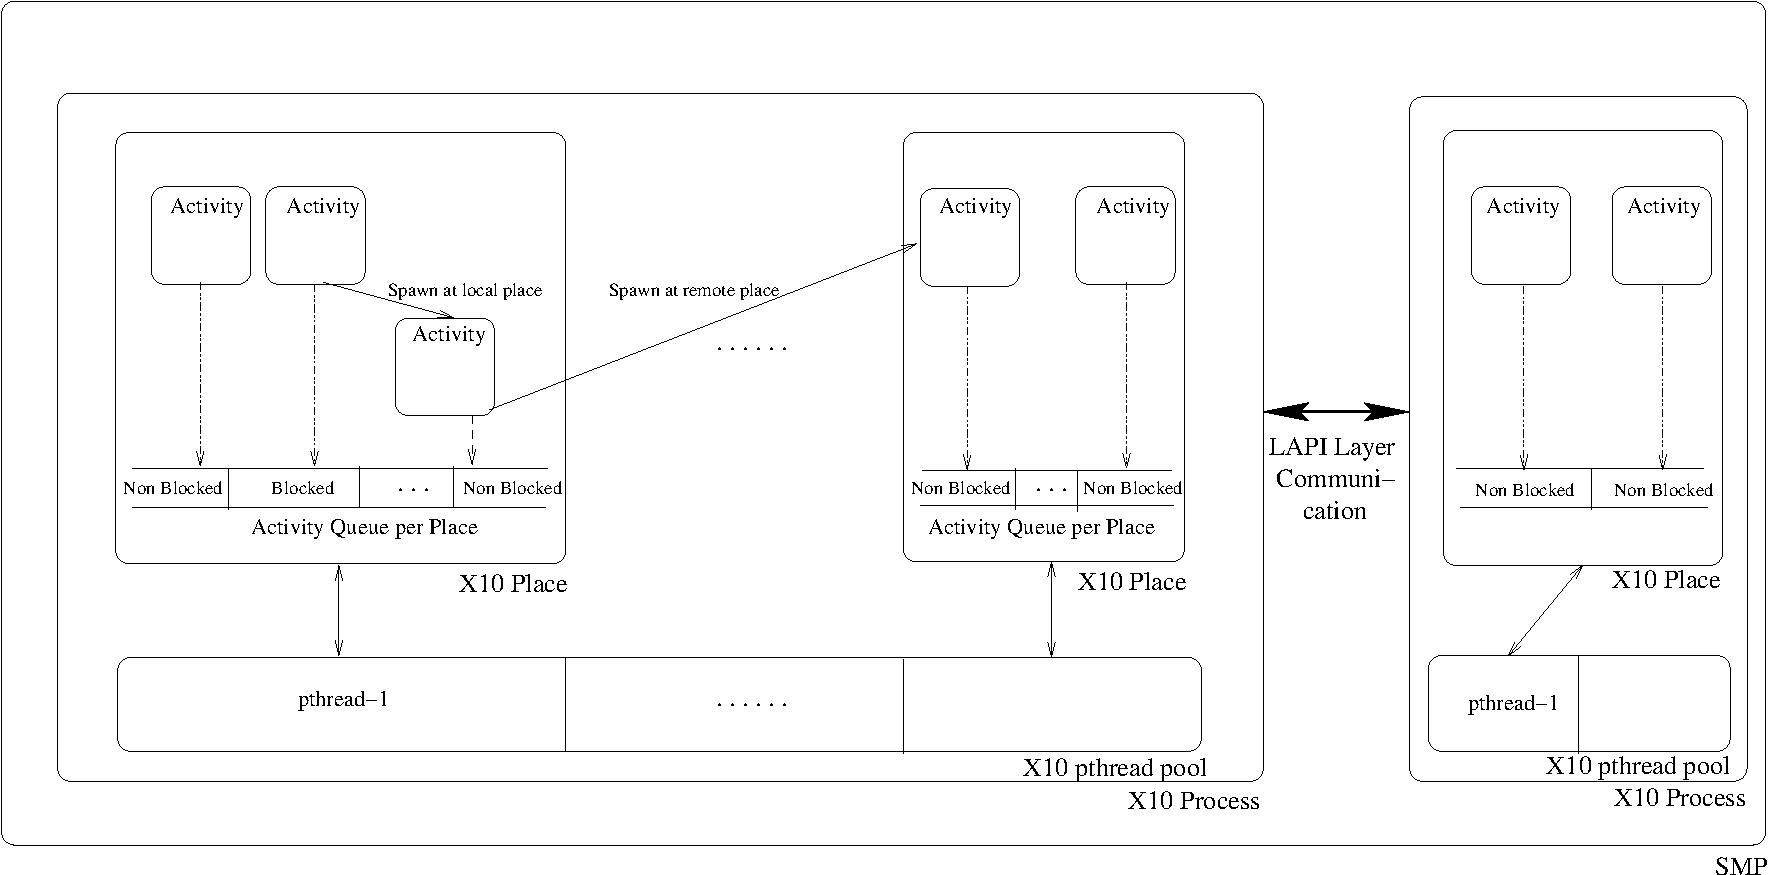
\includegraphics[width=\linewidth]{design-A}
\includegraphics[scale=0.5]{GAS}
\caption{\Xten{} The address space of an \Xtenlib{} process}
\label{fig:as_layout}
\end{figure}

The shared region of a process is divided into two regions -- {\em common} and
{\em hosted}. The higher $n$-bits of the 64-bit address (i.e. $a_{63-x}$
to $a_{63-x-n}$) are used to address the common section. Each process
will store its private data in the common section. For example, the
meta-data (region, distribution, base address) of a distributed array
and the {\em single} variables~\cite{yelick98titanium} are stored in the common
section.  So each processor will need to provide backing store
(through its virtual memory system) for this portion of the address
space. When the processor wishes to access the contents of a location
in this region of the address space --- it merely reads the location in
its local address space.

Now we divide up the remaining address space among the $2^p$ nodes by 
using the next $p$ higher-order bits (ie. $a_{63-x-n-1}$ to $a_{63-x-n-p}$)
to identify the node. The portion of the 
address space that is allocated to a given processor $P$ is said to be 
``hosted'' at $P$. We call the union of the address spaces hosted at each 
processor the ``partitioned address space.'' Thus the total shared 
address space is divided up into the partitioned address space and the 
common address space. The entire addres space is pictorially represented
in Figure~\ref{fig:as_layout}. 

Whenever a processor $P$ desires to read or write an address  $A$ in the 
partitioned address space, it first determines the processor $Q$ at which 
this address is hosted, and then asks $Q$ to read or write the address on 
its behalf (using LAPI remote gets and puts). Note that  $A$ is valid in 
$P$'s address space but will never be referenced. So $P$'s virtual memory 
tables will need to allocate real memory only to the portion of the 
address space that is hosted at $P$ or is common.

An advantage of such a representation is that address arithmetic can be 
performed locally. Suppose that a processor wishes to get the contents 
of $A[i]$. The code will read the metadata for $A$ from locations in the  
Common Address Space. Using this information (e.g.{} information that says 
the array is block distributed, and provides the block size), the code 
will compute the target address for $A[i]$. Note that the code sequence 
necessary to do this calculation is {\em identical} across all nodes. Now 
that the target address is known the code will determine whether it is 
local or remote by examining the higher order bits. If it is local then 
it reads the location from its local memory, otherwise it uses a 
LAPI-get to read the memory.

It is not required that the contents of memory in the common address
space are actually identical across all processors.  Often they will
be. But sometimes they will be different. For instance, in the case of
global array A, the meta-data will be stored in the common
address space. The first (64-bit) word at this address will contain a pointer
into the portion of the partitioned address space hosted at this node
which contains the data for the local portion of the array.
Subsequent words may contain the meta-data for the array -- the
contents of these words may be identical across all nodes.

The point is that an address in the Common Address Space ``means'' the 
same to all processors, e.g. the global array A represented by the 
address 0x000078ABCDDDDDD in the Common Address Space. So processor $P$ 
can send a message to any other process $Q$ with this address, and $Q$ will 
be able to use it to get to its local data for $A$. The contents of the 
first word at this address will be {\em different} for each processor $Q$ -- 
but will mean ``the same,'' i.e the local portion of the array.

\subsubsection {Implementation}

The new operator in C++ should be overloaded and thus transparently
(i.e. without explicitly telling at an allocation site) use a custom
memory allocator for objects of certain types. 
A sufficiently large chunk of the address space is allocated ahead of time 
using a special OS call (e.g. {\bf mmap})~\cite{gasnet}. The distributed objects and arrays 
are placed in this large chunk as the program executes.  
The custom memory allocation for PGAS implementation (done in C++ or
C) is useful for two reasons.

First, depending on the communication subsystem (e.g. LAPI) virtual
memory pages that belong to the PGAS may have to 'pinned', i.e. marked
to stay resident in main memory. This is necessary to serve remote
accesses timely without the risk that a remote access hits into
virtual memory that is paged out. 

Secondly, one can allocate the chunks of a distributed array in
different nodes at the same address offset. If both contiguous array
variables are allocated at the same offset in the virtual address
space in each node, then the computation of the virtual address of any
array variable can be done easily at the source node without any address
translation at the home node.

\subsubsection {Remote References}

In shared memory systems where all accesses to data are through global
pointers, all pointers are valid at all places. In such a scenario,
the programmer can separate the problems of data distribution and
computation partitioning. This greatly simplifies programming. In a
distributed memory machine the shared memory abstraction incurs a
performance penalty. This can be reduced by automatically translating
global pointers to local pointers where possible.  In the context of
\Xten, every pointer carries the place of residence in its type. The
compiler can translate global reference to local references. Asyncs
that are thus determined to operate on local pointers can be inlined.

The runtime does not provide any such support and requires the user to
explicitly distinguish local and remote references. In \Xtenlib, remote
references encapsulate global pointers, potentially making them
safer. In a typical one-sided library, global pointers are identified
by a place id and a pointer at that place. These two components are
visible at all places, potentially allowing dereference of a remote
pointer at the current place, resulting in undefined behavior.

\Xtenlib{} allows access to the pointer encapsulated by a global pointer,
only if that global pointer is local, i.e., points to a data structure
at the current place. This prevents accidental dereference of the
global pointer at an incorrect place. To access an address that is not
local (i.e. read or write), LAPI put/get methods should be used. 
\subsection{Deployment}
\label{sec:deploy}

A key feature in \Xten{} programming model is the concept of {\it
places} which establishes a mapping between a set of {\it activities}
and a set of locations in the partitioned global address space({\it
PGAS}). The mapping of places to physical processors and memory is
known as {\it deployment}. The {\it deployment} scenario plays a vital
role in the design of efficient \Xten{} execution environment. In this
section, we will discuss on efficient \Xten{} runtime design choices
for deployment in a cluster of SMP nodes.

An \Xten{} program written using multiple places can emulate multiple
places within a physical SMP node. Various design choices can be
thought of:

\begin{itemize}
\item A set of \Xten{} {\it places} are deployed in a single SMP node.
Each \Xten{} place is assigned exactly one pthread for computation.

\item A set of \Xten{} {\it places} are deployed in a single SMP node.
A set of \Xten{} places are assigned one pthread for computation.
\end{itemize}

In the first iteration, we will be considering the first choice i.e.,
each \Xten{} place is deployed on one pthread of an SMP
node. Figure~\ref{fig:deploy1} is a pictorial view of the activities
executing within a single SMP node. An \Xten{} job consists of a set
of \Xten{} processes. The mapping from processes to processor cores in SMP
is provided in the configuration file. Each \Xten{} process hosts an
\Xten{} place. Each \Xten{} place is associated with an ``unbounded'' 
activity queue which keeps track of both {\it blocked} and {\it
non-blocked} activities. Blocked activities will be tagged and will
not be selected for execution until they are untagged by the predicate
of the data structure on which it is blocked. Non-blocking activities
continue execution till completion. When there are activities in the
activity queue, the \Xten{} process pool executor will pick the top
most activity from the queue and assign it to the designated pthread
for execution.  If the executing activity is non-blocking, it executes
to completion. However, if the activity is blocking, it will be tagged
as ``blocked'' on a predicate of a data structure and is put back in
the queue when it is awakened by the same data structure. Activities
of a \Xten{} place are allowed to create both non-blocking and
top-level blocking activities at remote places.

\begin{figure}
\center
%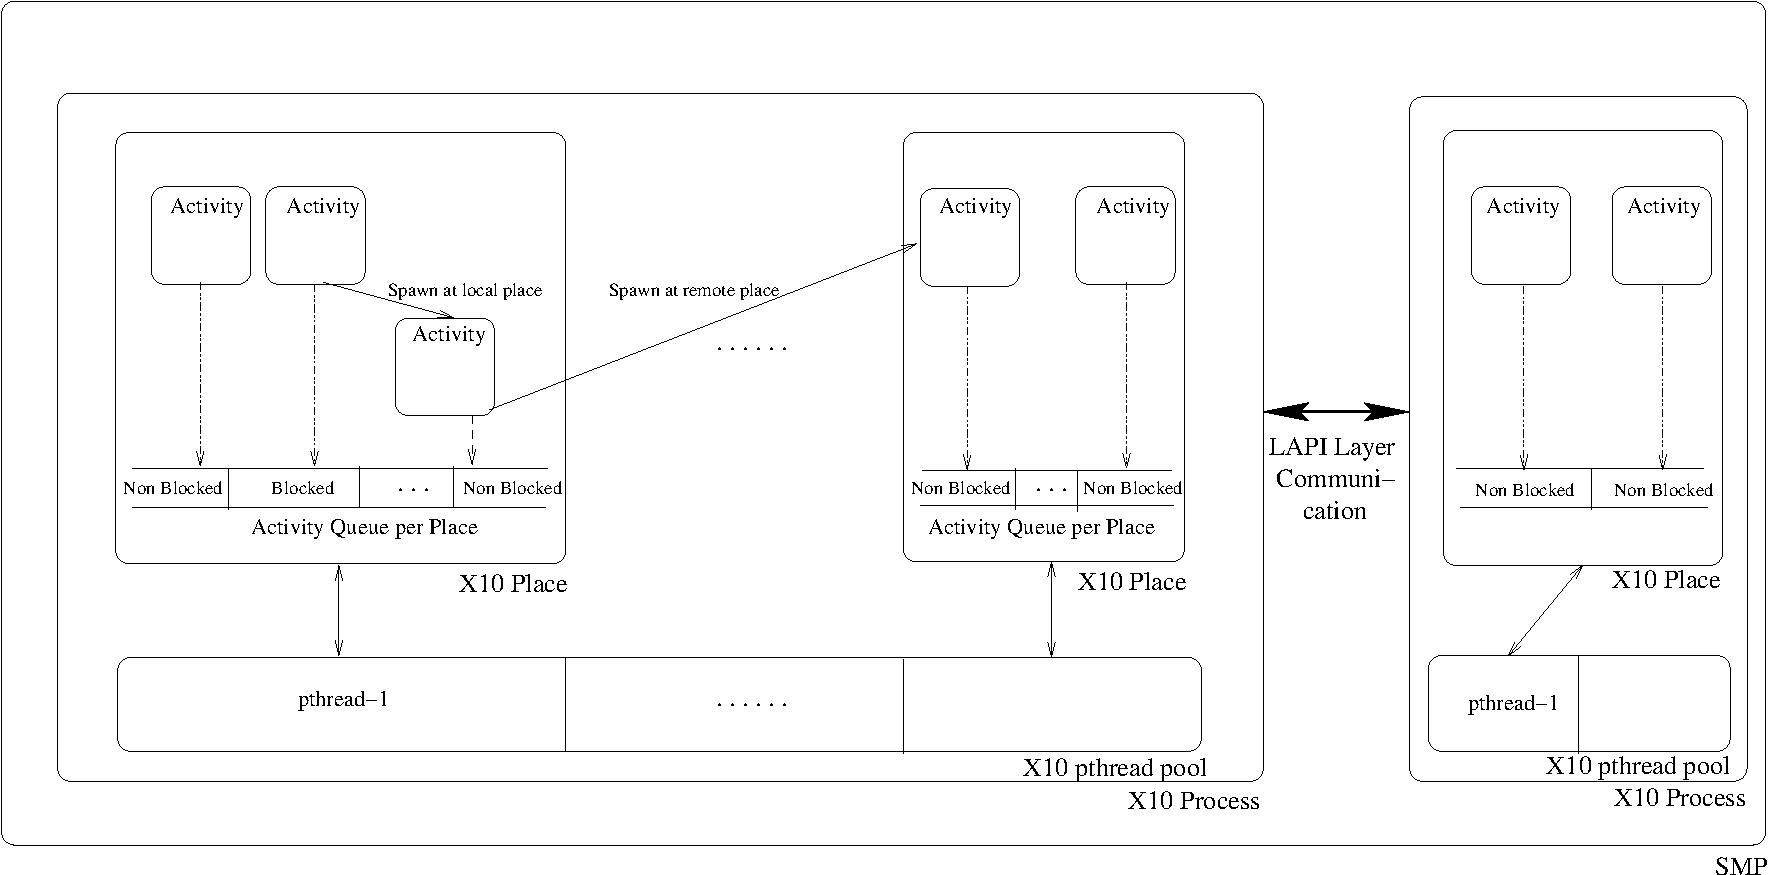
\includegraphics[width=\linewidth]{design-A}
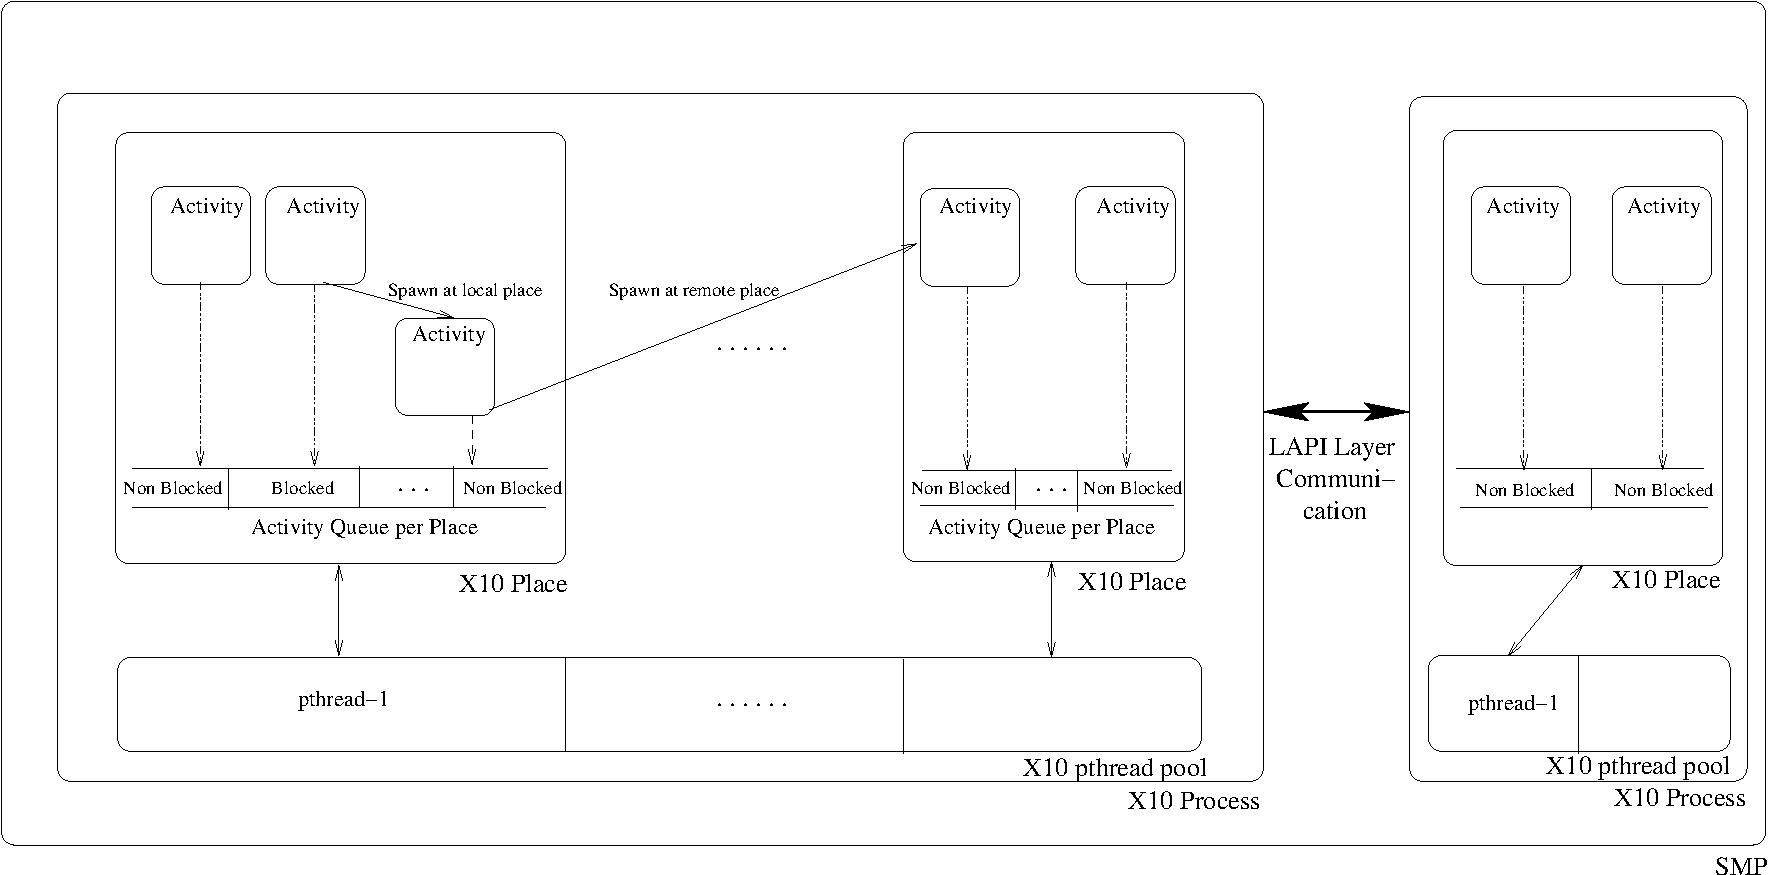
\includegraphics[scale=0.5]{design-A}
\caption{\Xten{} deployment on an SMP node}
\label{fig:deploy1}
\end{figure}

\subsubsection{Activities}
\Xten{} programming model allows activities to be either place local
or remote.  These activities can execute any arbitrary code within its
body including blocking operations. The blocking property of an
activity is derived from the fact that it uses one of the following
\Xten{} constructs in : {\it finish}, {\it future-force}, {\it
clock-next}, and {\it atomic-blocks}. In the first iteration, we will
allow top-level blocking activities  and non-blocking activities. Note
that top-level blocking activities are those which does not have a
predicated wait in method body. This information can be determined statically.

Local non-blocking activities may execute like an ordinary function
call.  The compiler may inline such activities.  Local blocking
activities are enqueued in the local activity queue for
execution. During the course of execution if the activity blocks, it
suspends its execution and waits on a predicate of a data structure to
be set. As soon as the predicate of the data structure is set, the
blocked activity is again enqueued and allowed to continue its
execution. Remote blocking activities are enqueued at the destination
place's activity queue and follow the same semantics of blocking as
local blocking activities. Remote non-blocking activities are enqueued
at the destination place's activity queue.


{\bf Operations on Activities:}


\begin{itemize}
\item {\bf Spawning new activities:} New non-blocking child activities
are always allowed to be created. Similarly blocking child
activities are allowed only if they do not have conditional wait in
method bodies. Note that arbitrary blocking activities are not
considered in the first iteration.
\item {\bf Executing blocking operation:} Mark the activity as
blocked in the activity queue  and allow other activities to progress.
\item {\bf Re-enabling blocked activities:} When the predicate of the
data structure is set, the blocked activity is re-enabled in the
activity queue and allowed to proceed with the execution.
\item {\bf Registration on clocks:} Activities during creation or
execution can register with clocks. Clocks keep track
of all activities that are registered on them at a given point of
execution.
\item {\bf Deregistration on clocks:} During execution, activities can
deregister themselves from certain clocks by explicit API calls. This will
implicitly mean that these activities will not participate in
subsequent clock quiescence. 
\item {\bf Resume on clocks:} When an activity invokes {\it resume}
operation on a clock, it intends to say that it has finished
computation of the current phase and moves to the next phase. 
\item {\bf Waiting for clock quiescence:} Activity invoking {\it
next} operation needs to wait for  global quiescence of all clocks
that it is registered with.
\item {\bf Critical region code execution:} Codes protected under
atomic sections are executed exclusively with respect to other
activities within the context of a \Xten{} place. 
\item {\bf Propagate exceptions:} During execution an activity can
throw exception which will be propagated to the innermost {\it finish}
scope.
\item {\bf Collective operations:} A set of activities can participate
in performing an operation collectively i.e., finding the sum of a
distributed \Xten{} array.
\end{itemize}


{\bf Example:}\label{sec:deploy:example}


Consider the following code fragment from RandomAccess benchmark
of HPC Challenge benchmark suite:
\begin{verbatim}
1: finish ateach (point p[i]: ranStarts.distribution) {
2:    long ran = nextRandom(ranStarts[i]);
3:    for (point count: [1:N_UPDATES_PER_PLACE]) {
4:       final int j = f(ran);
5:       final long OK = smallTable[g(ran)];
6:       async(table.distribution[j]) 
7:           atomic {
8:              table[j] = table[j] ^ OK;
9:           } 
10:      ran = nextRandom(ran);
11:   }
12:}	 
\end{verbatim}

The above piece of code updates the {\it table} elements based on a 
randomly computed index. There are two distributed \Xten{} arrays:
{\it ranStarts} and {\it table}. Elements of these arrays are
distributed in the partitioned global address space and is shared
across  SMP nodes, \Xten{} processes, \Xten{} places and \Xten{} 
activities.  Statement~1 creates a number of 
asynchronous activities at various places based on the distribution of 
{\it ranStarts} points. Each of these activities subsequently update
the {\it table} elements in Statements~6-9. The number of updates at 
each place is bounded by a constant {\it N\_UPDATES\_PER\_PLACE} in
Statement~3. Note that {\it smallTable} is not distributed and all 
of its elements are resident in a fixed predefined initial place.
Since the updates to table elements are performed across various \Xten{}
places, Statement~8 is protected in {\it atomic} sections in
Statement~7.


\subsubsection{Atomics}
Atomic sections are implemented using locks. Each place will have 
a set of locks.  An activity may request to 
perform an atomic operation at a place which in turn will be
translated to obtaining the locks at the designated place before
performing the operation. These locks are globally ordered,
precluding deadlocks. Obtained locks cannot be passed from one
activity to another, and all locks required by an activity need to be
obtained together. 

On a cluster of Power5 SMP nodes, we primarily have two types of atomics: {\it
primitive} atomics and {\it compound} atomics. {\it Primitive} atomics
do not block within the same SMP node and use {\tt lwarx} and {\tt
stwcx} instructions to atomically update within a SMP node. However,
across SMP nodes, we need {\it compound} atomics which explicitly
obtains lock at the designated place to perform the operation and are
blocking in nature. It can be observed that primitive atomics designed
specifically to improve performance on a cluster of Power5 SMP nodes.

Consider the RandomAccess code fragment given in
Section~\ref{sec:deploy:example}. The spawn of asynchronous activities
in Statement 6 can be optimized to leverage the {\it primitive}
atomics concept on Power5 and can get rid of the cost of creating 
new asynchronous activities and obtaining locks within the same SMP
node.


\REM{
Support for conditional atomics is provided. A special type of
variable, a {\tt WatchedVariable}, may be declared and allocated on
the heap. An async may be attached to a {\tt WatchedVariable},
together with a triggering {\tt CallRecord}. The triggering {\tt
CallRecord} must be pure, that is it must have no
side-effects. Typically it will simply check the value of the variable
and return true or false. Triggers are evaluated whenever the value of
the {\tt WatchedVariable} is set. If the trigger evaluates to true, the
trigger is removed and the associated async is executed (or scheduled
for execution).
}

\subsection{Arrays}

\Xten{} arrays provide support for the creation and manipulation of
distributed multi-dimensional arrays. Once created, any activity can
operate on arbitrary regions of the array, potentially through asyncs. The
implementation of \Xten{} arrays in \Xtenlib{} will provide the
interface for all \Xten{} array operations viz., point-wise, reduction,
scan. Also, an efficient iterator function will be provided. The maximum rank
(i.e. the number of dimensions) of the array supported by
the library will be fixed to a small constant (say 7). 

A distributed array consists of two key components -- meta-data and
data. The meta-data consists of information about the array, like,
shape (rank and size of each dimension), distribution etc. 
The meta-data is stored in the local heap of each process and
is immutable.
The data consists of the actual array data. The data is allocated
in the hosted address space of each process. The meta-data and
data are referred to as {\tt array\_info} structure.  

We categorize the distributed arrays into three kinds -- {\em regular},
{\em semi-regular} and {\em irregular}. The regular arrays are created
only by the root process (ie. the process that executes the first
activity) and have very regular distribution -- that is,
all the processes own a chunk of data and the chunks are of same size
in all the nodes. Semi-regular arrays satisfy the property that it can
be allocated by the root process; the other two properties of regular array
do not hold. Irregular arrays are the most
general arrays which don't have any of the above 3 constraints of the 
regular arrays. For efficiency in array access operations,
we plan to allocate each of these arrays differently.

\subsubsection{Regular Arrays}
\begin{figure}
\center
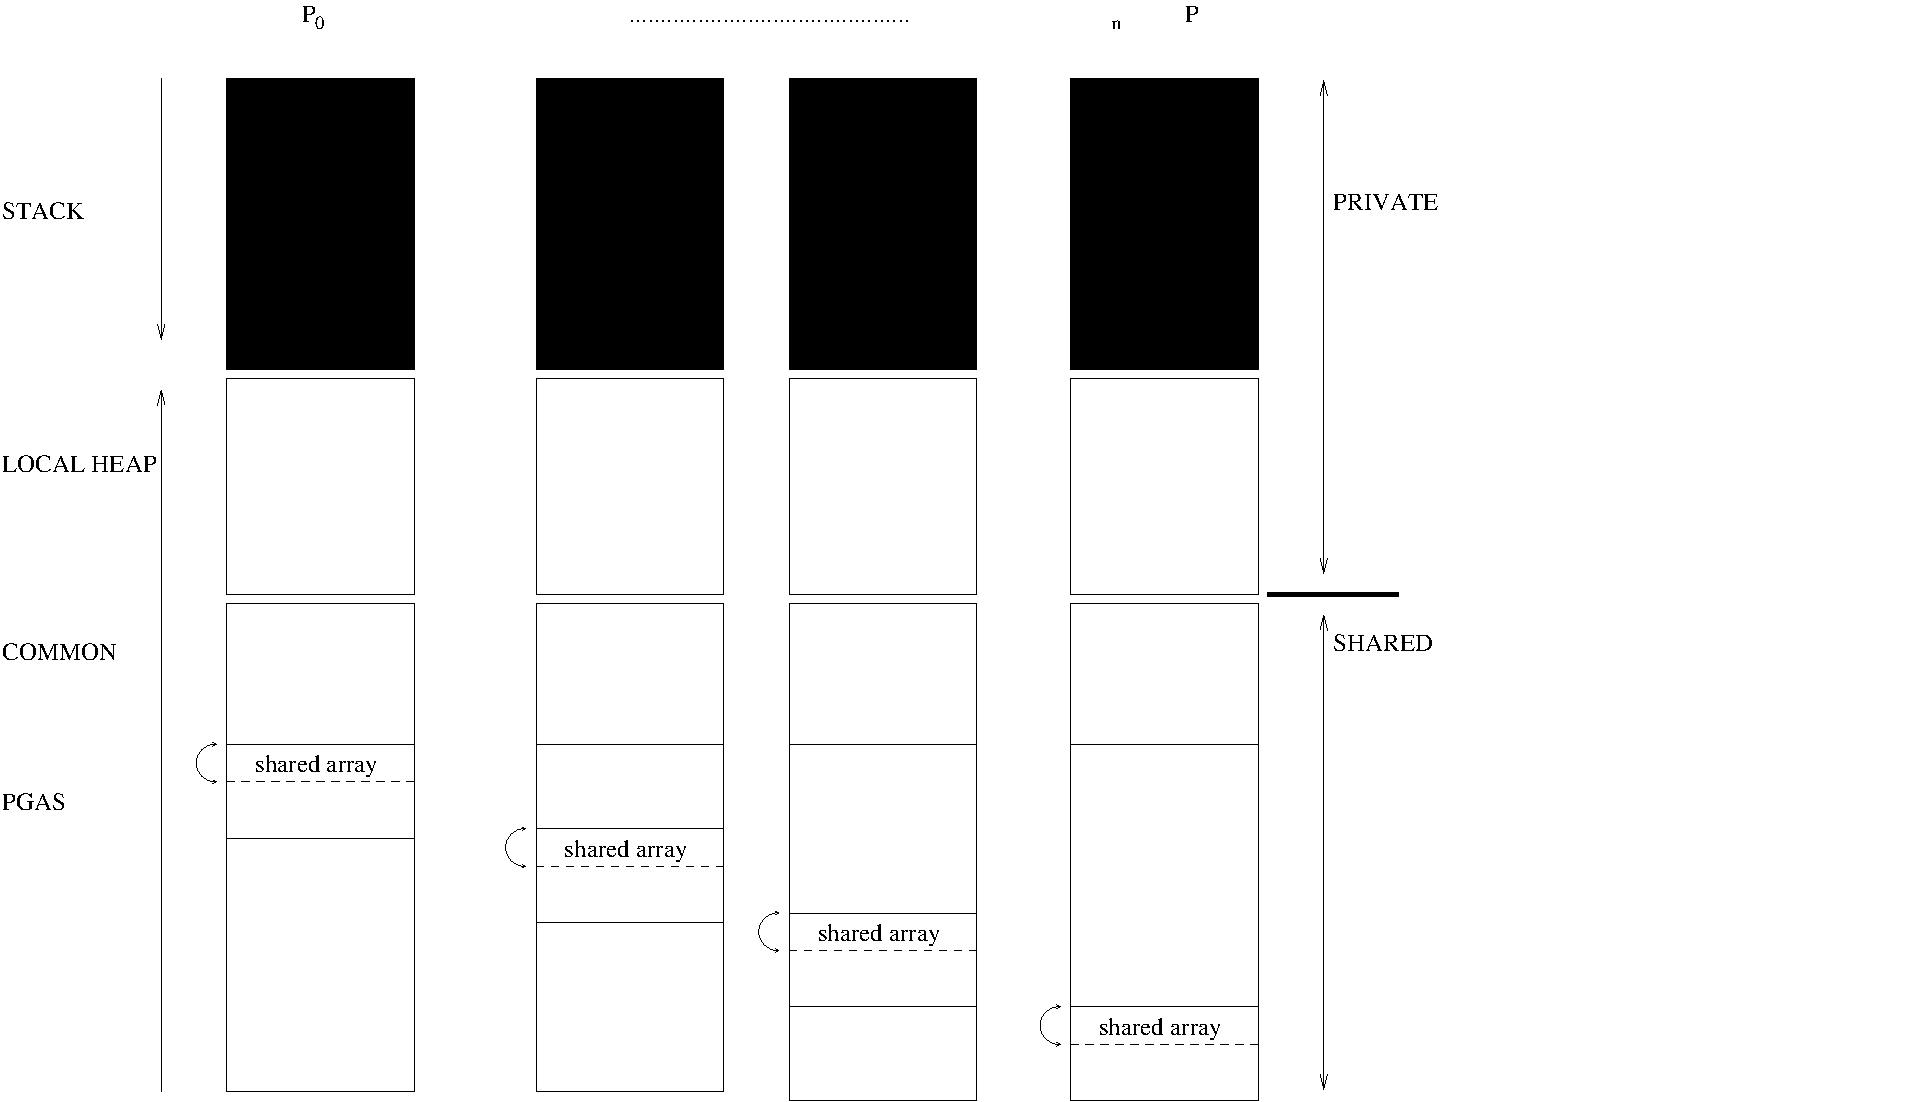
\includegraphics[scale=0.5]{ARRAY-REGULAR}
\caption{A sample layout of a {\em regular} distributed array}
\label{fig:array_layout_regular}
\end{figure}

For regular arrays, we plan to exploit the benefits of GAS and the compiler.
The chunks of regular arrays are allocated in a special region called {\em array}
region. This array region is a part of the PGAS. All the process allocate its
chunk in the same base address, with the first word containing a pointer to 
the meta-data. The rest of the words contain the data. This allocation scheme is shown in Figure~\ref{fig:array_layout_regular}.

The main advantage of this allocation is that an array access like $a[i]$ will
be directly compiled to the following target code by the compiler : $get(((a.base \& mask) | node\_id) + local\_offset(i))$.
Thus, no extra table lookup is required, unlike the allocation scheme that we will see in the following
sections.

Consider again the RandomAccess code of Section~\ref{sec:deploy:example}. The code
has two distributed arrays - {\tt table} and {\tt ranStarts}. Both these arrays
are created in the beginning of the program as follows:

\begin{verbatim}
1: final long[.] table = new long[block(TABLE_SIZE)] 
2:               (point p[i]) { return i; };
3: final long[.] ranStarts = new long[unique()]
4:		(point p[i]) { return C.starts(N_UPDATES_PER_PLACE*i); };
\end{verbatim}

The root process invokes the array constructor. The array constructor
determines the base address where the array needs to be allocated. It then
sends a message to all the processes to allocate the array at the same
base address in their section of PGAS along with initial data
and meta-data of the array. The processes receive the message,
allocate the array and initialize it. The array construction terminates only
after the message is received and the arrays are allocated and initialized
at the receiving end.

\subsubsection{Semi-regular Arrays}

\begin{figure}
\center
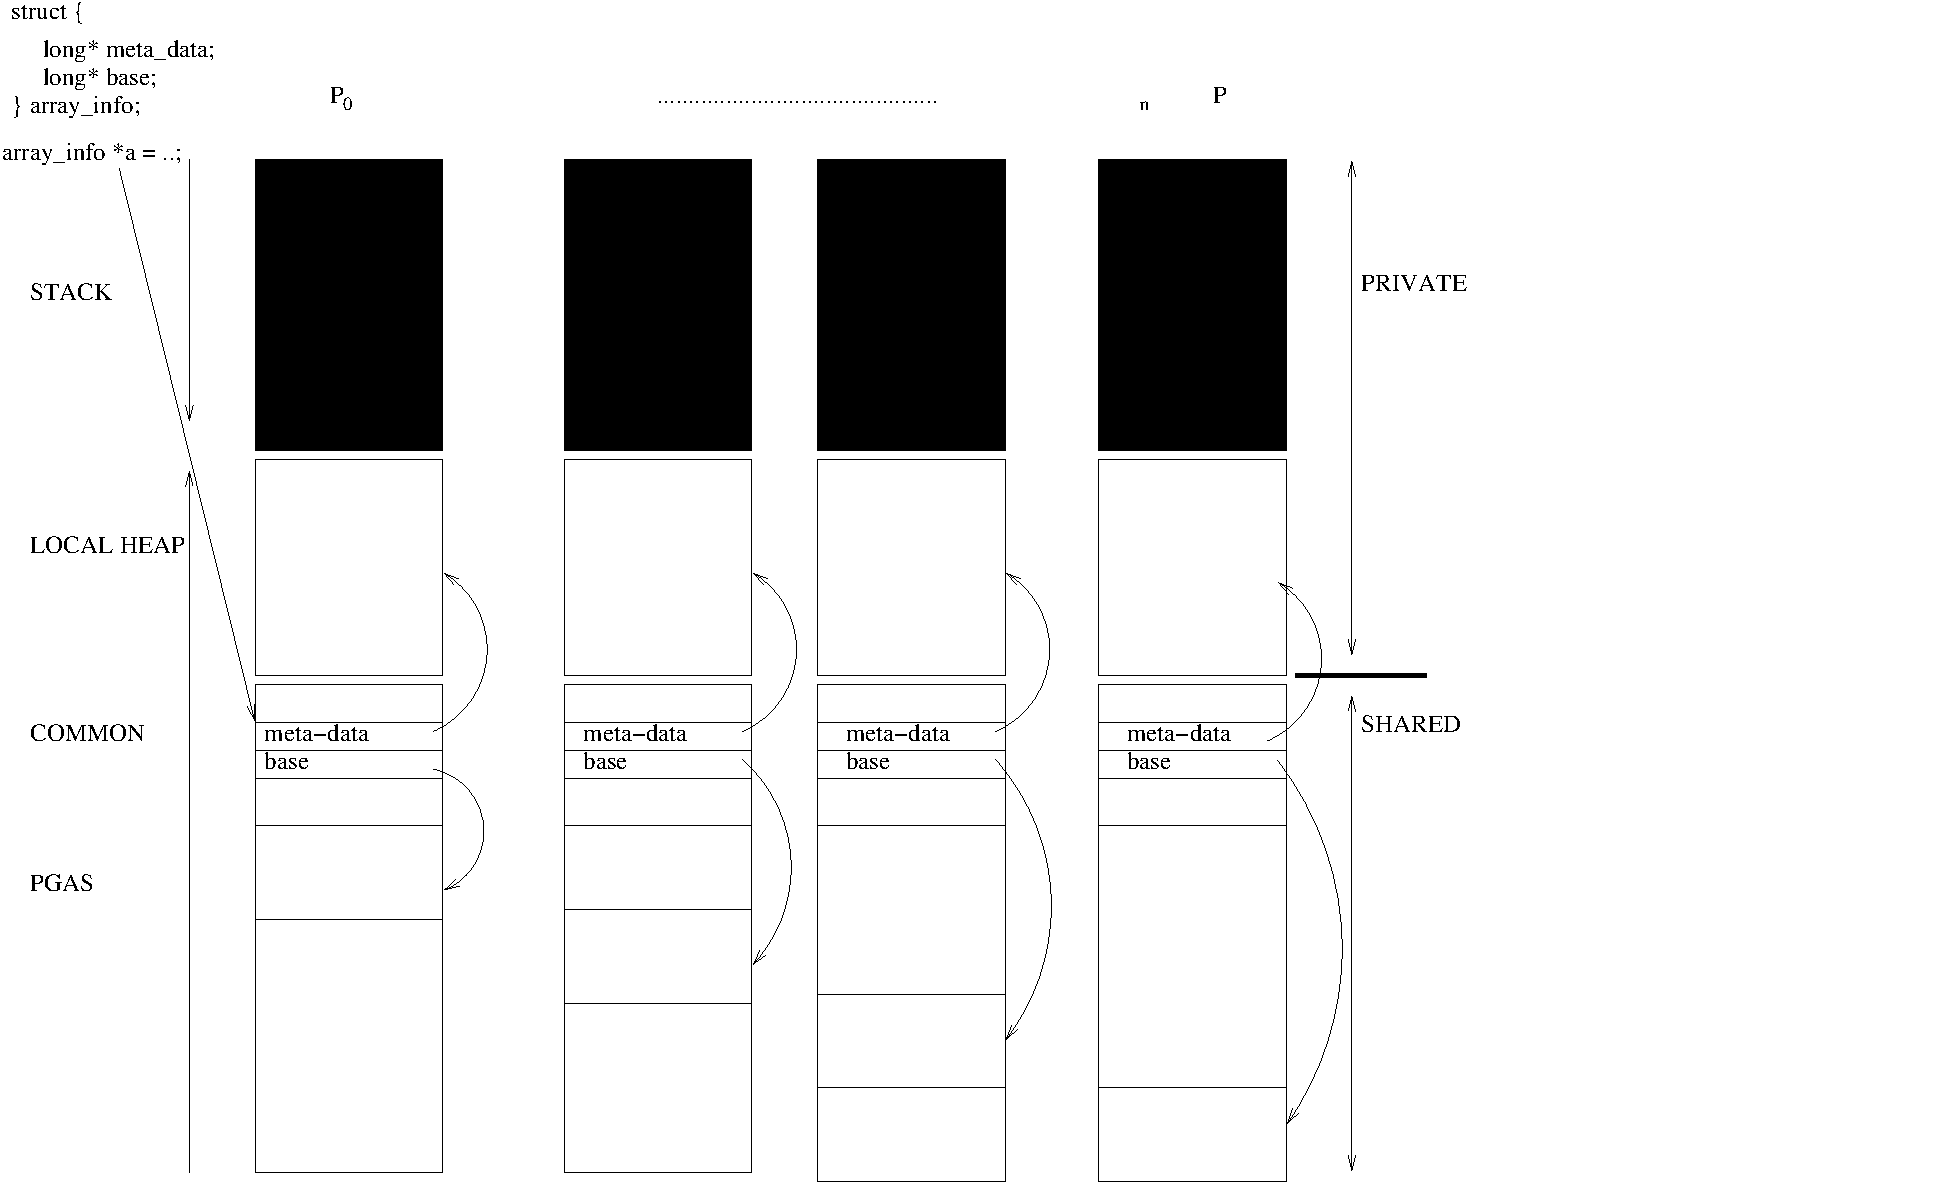
\includegraphics[scale=0.5]{ARRAY-SEMI}
\caption{A sample layout of a {\em semi-regular} distributed array}
\label{fig:array_layout_semiregular}
\end{figure}

For semi-regular arrays, the
{\tt array\_info} is stored in the common address space. The root process
sends a message to all the process to allocate the {\tt array\_info}
in the same address. Upon receiving this message, each processor
allocates the space for {\tt array\_info} (in the common address space), meta-data 
(in the local heap) and data (in the hosted space). A sample layout of a
distributed array in the address space is shown in the Figure~\ref{fig:array_layout_semiregular}.

For example, in the RandomAcess code listed in the previous section, the root process
invokes the array construction. The root process sends
a (LAPI) message to each process requesting a block of the array to be allocated
on that process and initialized. Initialization information and other information like the distribution are sent to the
processes in the message. 
Upon receiving the message, each process creates a meta-data for the array
in its local heap, and allocates a region in its hosted address space (cf. Section~\ref{sec:gas})
for the local data section of the array. It also stores the {\tt array\_info}
in the address sent by the root process in the common address space. 
The call to the array creation routine returns only after the message
is received by the processes involved, and the array sections are initialized
in each process. 

\subsubsection{Irregular Arrays}

\begin{figure}
\center
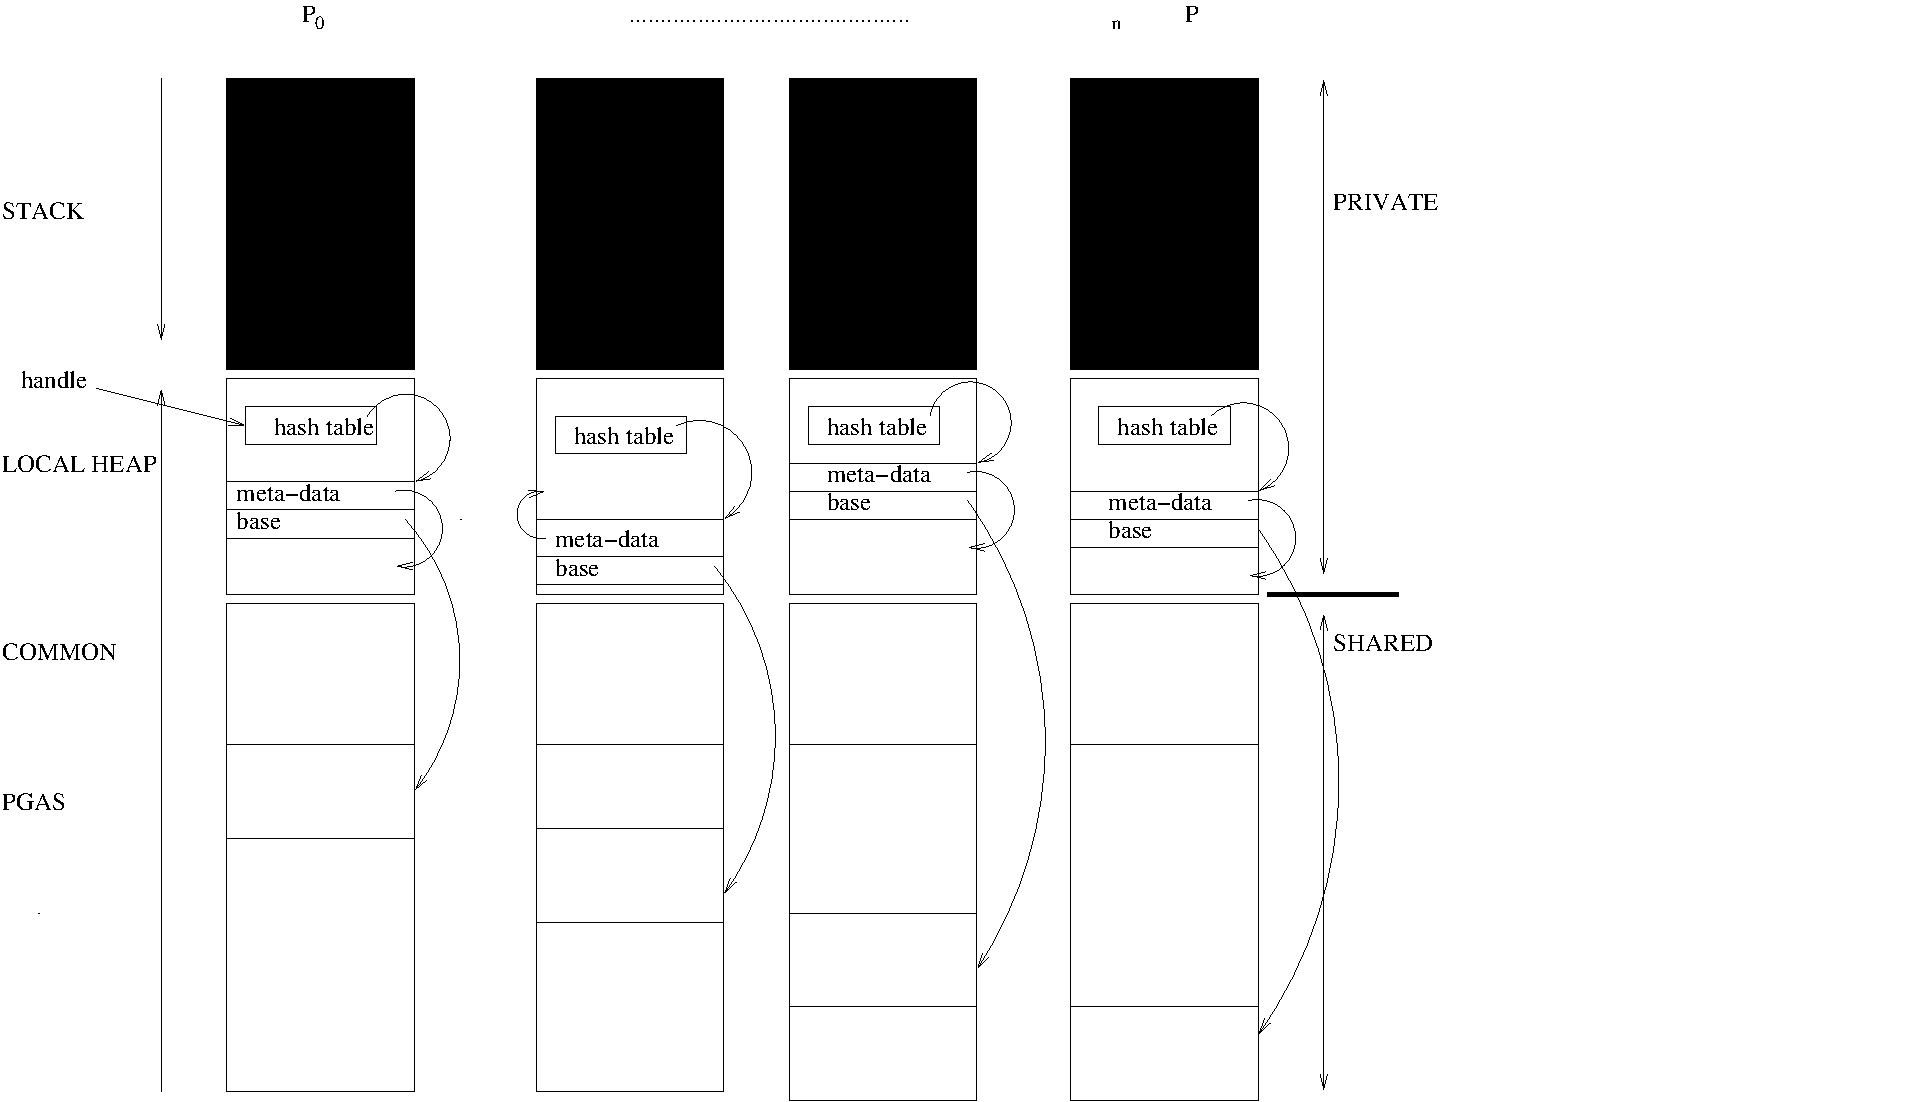
\includegraphics[scale=0.5]{ARRAY-IRREGULAR}
\caption{A sample layout of an {\em irregular} distributed array}
\label{fig:array_layout_irregular}
\end{figure}

Irregular arrays are the most general arrays. For these arrays, we generate
a unique handle to represent the distributed array. This unique handle
can be generated by the concatenation of process ID and a local counter.
(ie. $\langle$process id,local counter$\rangle$). A hash-table is allocated
in the local memory of each process. The unique handle is used to lookup in to
the hash table and obtain the {\tt array\_info} for the given handle (array). 
This scheme is shown in the Figure~\ref{fig:array_layout_irregular}.

For example, in the RandomAccess code, the activity that creates the 
arrays (not necessarily the root activity), constructs an unique handle
using the above mentioned scheme. It then sends this handle and other
information (initial values, meta-data etc.) to the other processes
that need to allocate a section of the distributed array. On the receiving 
end, each process allocates the {\tt array\_info} in its local memory.
The data for the array is allocated in their section of PGAS. The pointer
to the {\tt array\_info} is stored in the hash table entry corresponding
to the unique handle sent by the activity that invoked the array constructor. 

%In architectures such as BlueGene/L, without native support for RDMA,
%identifying the local buffer base address at the remote node is
%efficient. This is how the implementation of shared value directories
%is done in UPC on BlueGene/L~\cite{PLDI06}.  On architectures supporting
%zero-copy RDMA, \Xtenlib{} combines the above approach with a cache of
%shared array information on remote nodes on which they were recently
%accessed. Thus the first communication is expensive, being implemented
%by a remote activity, but subsequent remote memory access is through
%optimized put/get operations.

%Another design alternative is to choose the base address of the local section of the array to be
%same on all the nodes. This might involve an all-to-all communication among
%the nodes to decide the common base address. Since \Xtenlib{} provides the 
%global address space (GAS) abstraction (Section ~\ref{sec:gas}), choosing a common base address is a
%natural way to represent shared arrays.

%Prevalent runtime systems create shared arrays collectively.  Each
%process assign an index in a meta-data table for the shared array
%being created. Assuming all processes are involved in the shared array
%creation and they do so in the same order, all processes can decide on
%the same entry index in the local meta-data tables. This index is used
%as the globally unique handle.

%\Xtenlib, supporting the non-collective shared array creation, uses a
%$\langle$place id,local counter$\rangle$ from the creating activity as
%the shared array handle. Unlike in typical implementations in which
%the shared arrays handles index into a table, they index into a hash
%table.

%\subsection{Additional intrinsics}
Additional functionality provided for spawning of activities on all
places, and efficient put/get operations using LAPI.

\subsection{Execution Environment}
There are two modes of using the \Xtenlib{}. In the first mode, the
compiler compiles the \Xten{} source program and links it with the
\Xtenlib{}.  The programmer issues a command to execute the resulting
executable using a script.  The script is responsible for sending the
executable across the network to each of the SMP nodes. The script
also reads a configuration file.  The contents of the file will
specify how many processes need to be created for this computation,
the hosts on which these processes need to be run, the number of
places to be created in each process, and the number of threads to be
created for each place.  The root activity will be run by a master
thread.  The other threads in each process will suspend waiting for
incoming asyncs. By a thread, we refer to the application level
threads, which may or may not be the same as a {\tt pthread}.

\Xtenlib{} is available for direct use by programmer too, following MPI style operation.
The programmer is responsible for writing an SPMD-like code that uses
the \Xtenlib{} intrinsics. {\tt X10::Initialize()} initializes the
runtime system in each MPI process, and {\tt X10::finalize()} performs
any necessary clean-up. All invocations of X10 API must be after
initialization and before clean-up.  The X10 runtime object at the
current place is implemented as a singleton, and is accessible by the
{\tt TheX10()} method.  A place is identified by an integer. The
number of places is fixed and does not change during the
execution. Methods {\tt TheX10::here()} and {\tt TheX10::maxPlaces()}
return the current place id and the number of places.






\section{Conclusion}
\section{Conclusion}\label{s:concl}

\paragraph{Acknowledgements.} \XWS{} is being designed and implemented in collabration with Doug Lea. We thank Raj Barik for his contributions to the implementation of the C++ version of \XWS. We thank the rest of the X10 team for many discussions of these issues.
%\section{Future Directions}
%%V. Conclusion and future work. (0.5 page)
%
%state-dependent constrained types.
%
%use of dependent types for optimization. 
%
%type-inference.
%
%Bibliography (1.5 page)

We are actively writing programs with constrained types in
\Xten{} and 
working to extend the expressive power of the type system.
In particular, we are focusing on the following extensions:

\paragraph{Driving optimization.}
\paragraph{Clocks.}
\paragraph{Type constraints.}
By allowing classes to have type properties as well as value properties,
and by incorporating subtyping constraints into the language, we believe we can achieve the expressive power of generics.

\paragraph{Type inference.}  Constrainted types can be burdensome for
programmer to write down.  A type inference algorithm for constrained types.

\paragraph{Flow sensitivity.}  The following code should type-check:
\begin{xten}
int x = ...;
int(:self >= 0) y;
if (x >= 0) {
    y = x;
}
\end{xten}

\paragraph{State-dependent constrained types.}



%\section{Hello World Example}
%
\begin{verbatim}
#include <iostream>
#include <mpi.h>
#include <x10.h>

using namespace std;
using namespace X10Runtime;

class HelloWorldActivity : public Activity {
public:
  class Maker: public ActivityMaker {
    public:
      Activity* make() {
        //scope - finish scope from ActivityMaker
        return new HelloWorldActivity(scope); 
      }
  };
  HelloWorldActivity(const FinishScope &scope) : Activity(scope) {}
  ProbeStatus run() { 
    cout<<"Hello World"<<endl; 
    return acDone; 
  }
};

int main(int argc, char *argv[]) {
    MPI::Init(argc, argv);
    X10::initialize();
    TheX10().process(HelloWorldActivity::Maker());
    X10::finalize();
    MPI::Finalize();
}
\end{verbatim}

\appendix
\section{Background}
\subsection{\Xten}
The \Xten{} language provides support for a non-SPMD style
functional-parallelism oriented programming. The unit of parallelism
in an \Xten{} program is an {\em activity}. The \Xten{} computation
starts with a single activity. Activities execute in {\em places}; a
single \Xten{} computation runs over many places, scattered over
multiple nodes in a cluster. Activities are resident in the place in
which they are created, and they can read and write data in the place
in which they run. The may also create new local data items. Data
items once created do not move. An activity can spawn other activities
to be executed in parallel in the current place or in other places.
All access to remote data is through activities and serialization of
remote objects.

An activity may also create a global data-structure, such as a global
array. Such a data-structure has state scattered across multiple
places. Operations on the data-structure may be invoked by an activity
in any place and typically result in computation across many places.

Of particular interest in \Xten{} are distributed arrays. These are
organized around a {\em region} -- a data-structure representing the
set of {\em points} over which the array is defined -- and a {\em
distribution}, a partitioning of the region over some subset of
places. Sometimes the programmer may wish to operate upon an array in
parallel using multiple activities within the same place; in this case
a {\em tiled region} may be used to divide the array up between these
activities. A tiled region is an array of regions. (In subsequent
versions of the language we intend to introduce hierarchically tiled
arrays.)

{}\Xten{} supports a notion of {\em immutable} data. Objects that are
immutable may may be freely copied from place to place by the
implementation and are hence not associated with a particular place.

In addition to the activity-based communication model, \Xten{}
supports libraries for efficient copying of sections of arrays from
one place to another.

Finally, \Xten{} supports a few constructs for coordinating multiple
activities. As noted above, an activity may spawn multiple activities
in the same place or in other places. Further it may wait until all
activities spawned during the course of execution of a statement have
(recursively) terminated, using the {\tt finish S}
construct. Activities may use {\em conditional atomic blocks} for
synchronization ({\tt when (c) S}). Such a block permits an activity
to wait until a specified condition {\tt c} is true, and then in one
atomic step execute the statements in {\tt S} (in the same state in
which {\tt c} is true). Conditional atomic blocks are a very simple
and powerful synchronization construct, and can be used to elegantly
implement all the usual concurrency coordination idioms
(producer/consumer synchronization, mutual exclusion, barrier
synchronization etc). Of particular interest in \Xten{} are {\em barriers}


Atomic blocks are supported, with implicit locking.
\subsection{Messaging Passing Interface (MPI)}
MPI is a popular two-sided messaging passing communication
support. MPI-2 adds one-sided extensions, albeit with complex semantics. 
MPI is still primarily used as a two-sided library.
It is available on almost all high performance
computing platforms. Inter-operability with MPI can ease user
acceptance of \Xtenlib. In addition, \Xtenlib{} uses the process management
framework from MPI, i.e., an \Xtenlib{} program is started as an MPI
program.

\subsection{LAPI}

LAPI (Low-level API)~\cite{lapi} provides efficient remote memory access
mechanisms (one-sided communication).  The LAPI library provides basic
operations to ``put'' data to and ``get'' data from one or more
virtual addresses of a remote task.  LAPI also provides an active
message infrastructure. With active messaging, programmers can install
a set of handlers that are called and run in the address space of a
target task on behalf of the task originating the active message.
These handlers can be used to dynamically determine the target address
(or addresses) where data from the originating task must be stored.

LAPI may operate either in {\em polling} or {\em interrupt} mode. In the former, a
user pthread invoking a LAPI function may be temporarily borrowed to
send or receive messages. In the latter a dedicated single pthread
(created at initialization time) is responsible for handling message
send/receive traffic.


\subsection{ARMCI}

ARMCI is a portable communication library that provides one-sided communication facility. It provides the functions for
memory to memory transfer operations, accumulation, read-modify-write operations, memory allocation etc. 
The data transfer operations are available in the form of two noncontiguous operations : ARMCI\_PutV and ARMCI\_PutS.
ARMCI\_PutV uses general I/O vectors to describe the source and destination memory locations. This is useful
for transferring any kind of data, with even non-constant stride (e.g. triangular section of an array).
ARMCI\_PutS is useful for transferring strides region with constant strides. For more information on these
functions, refer to ~\cite{armci}.

ARMCI also provides two atomic operations : {\em accumulate} and {\em read-modify-write}. Accumulate operation
combines the local and remote data atomically : {\tt $x = x + a \times y$}. Read-modify-write updates a
remote {\tt integral} variable according to a specified operation and returns the old value.

ARMCI also provides a simple progress and ordering rules. The progress rule is
that all the ARMCI one-sided operations complete regardless of
the actions taken by the receiver. That is, there is no need for the remote
process to make occasional communication calls or poll in order to assure
that communication calls issued by other processes to this process can
complete. 

The ARMCI operations issued to the same destination process complete
in order. Operations issued to different processors can complete in an
arbitrary order. Additionally, when a  put or accumulate operation completes,
the data has been copied out of calling process memory but has not 
necessarily arrived at its destination. This is a local completion. A global
completion can be achieved by calling ARMCI\_Fence operation. 
\subsection {GASNet } 

GASNet (Global-Address Space Networking) is a network-independent and language-independent high-performance communication 
interface for use in implementing the runtime system for global address space languages. It provides
two layers of interface - core and extended. The core API is a narrow interface
based on the Active Messages paradigm. The extended API is an expressive
and flexible interface that provides medium and high-level operations on remote
memory and collective operations. 

The core API provides the active messages functionality. Active message communication is formulated as logically matching request and reply operations. Upon receipt of a request message, a request handler is invoked; likewise, when a reply message is received, the reply handler is invoked. Request handlers can reply at most once to the requesting node and only to the requesting node.
 The active message routines are divided in to three kinds based on the size of the message transfer : gasnet\_AMRequestLongM(), gasnet\_AMRequestMedimM() and
gasnet\_AMRequestShortM(). Corresponding reply routines are also provided. Additionally, an asynchronous version of long request is provided in the
form of gasnet\_AMRequestLongAsyncM().

A key feature in
the active message interface of GASnet is the ability for programmer to
supply several parameters to AM handlers, as  a part of the
AM message routines. The library internally communicates those
parameters to the receiver. This functionality is useful for 
implementing remote {\em async} activities. A remote {\em async} activity is just
a function call that has to executed on a place P. An {\em async} can also
access certain local variables (e.g. final variables) from the parent's
local stack. These variables can be passed as arguments to the function call.

The extended API provides memory to memory transfer operations in the form
of put and get. Both blocking and non-blocking versions are provided. The non-blocking versions do not complete the operation, but return a handle. A synchronization operation on the handle should be performed to complete the operation.
Additionally, register-to-memory transfer operations are also provided. 

\section{Notes for \Xten{} compiler writers}

\subsection{Garbage collection}
\subsection{Asyncs}
\subsection{Atomics}
\subsection{Arrays}


\bibliographystyle{plain}
\bibliography{x10}

\end{document}

